\documentclass[a4paper]{report}
% Shared preamble for the English probability and statistics documents.
% Based on the original course preamble. Compile with pdfLaTeX.
\usepackage[top=1.5cm,bottom=2cm,left=2cm,right=2cm]{geometry}
\usepackage[T1]{fontenc}
\usepackage{lmodern}
\usepackage[utf8]{inputenc}
\usepackage[english]{babel}

\usepackage{amsmath}
\usepackage{amssymb}
\usepackage{amsthm}
\usepackage{mathrsfs}
\usepackage{mathtools}
\usepackage{etoolbox}
\usepackage{tikz}
\usetikzlibrary{shapes.multipart,arrows.meta}
\usepackage{xcolor}
\usepackage{enumerate}
\usepackage[shortlabels]{enumitem}
\usepackage{hyperref}
\usepackage{version}
\usepackage{bbold}
\usepackage{fontawesome5}
\usepackage{fancyhdr}
\lfoot{}
\usepackage{natbib}
\usepackage{graphicx}
\usepackage{pdfpages}
\usepackage{authblk}
    
\usepackage{blindtext}
\usepackage{multicol}
\usepackage{collcell}
\usepackage{wrapfig}
\usepackage{blkarray}
\usepackage{cancel}
\usepackage{appendix}
\usepackage{float}
\makeatletter
\input{tex/assets/slashbox.sty}
\makeatother
\hypersetup{unicode,colorlinks,citecolor=red,filecolor=black,
  linkcolor=red,urlcolor=cyan}
\setlength{\columnsep}{1cm}
\pagenumbering{gobble}

\def\numtext#1{%
  \ifcase#1\or one\or two\or three\or four\or five\or six\or seven\or eight\or nine\or ten\or
  eleven\or twelve\or thirteen\or fourteen\or fifteen\or sixteen\or seventeen\or eighteen\or nineteen\or twenty\or Lots\fi}

\newcommand{\Byte}[1]{%
  \def\nodecontents{}%
  \foreach[count=\l] \k in {#1} {\xappto{\nodecontents}{\noexpand\nodepart{\numtext{\l}}\k}}%
  \node[rectangle split,rectangle split parts=8,rectangle split horizontal,draw] at (2,2){\nodecontents};}

\newcommand{\D}{{\mathrm{d}}}
\newcommand{\cE}{{\mathcal{E}}}
\newcommand{\cG}{{\mathcal{G}}}
\newcommand{\cX}{{\mathcal{X}}}
\newcommand{\cY}{{\mathcal{Y}}}
\newcommand{\cB}{{\mathcal{B}}}
\newcommand{\cF}{{\mathcal{F}}}
\newcommand{\cO}{{\mathcal{O}}}
\newcommand{\cS}{{\mathcal{S}}}
\newcommand{\cT}{{\mathcal{T}}}
\newcommand{\given}{\, \big| \,}
\newcommand{\cL}{{\mathscr{L}}}
\newcommand{\cD}{{\mathcal{D}}}
\newcommand{\cA}{{\mathscr{A}}}
\newcommand{\cP}{{\mathscr{P}}}
\newcommand{\cR}{{\mathscr{R}}}
\newcommand{\A}{{\mathcal A}}
\newcommand{\one}{\mathbb{1}}
\newcommand{\mathbbm}[1]{\mathbb{#1}}

\providecommand{\C}{}
\renewcommand{\C}{\mathbb C}
\newcommand{\R}{\mathbb R}
\newcommand{\Q}{\mathbb Q}
\newcommand{\N}{\mathbb N}
\newcommand{\T}{\mathbb T}
\newcommand{\F}{\mathbb F}
\renewcommand{\P}{\mathbb P}
\newcommand{\Z}{\mathbb Z}
\newcommand{\E}{\mathbb {E}}
\newcommand{\Pbb}[1]{\P\left( #1\right)}
\newcommand{\Ebb}[1]{\E\left[ #1\right]}

\newcommand{\lb}{\left (}
\newcommand{\rb}{\right )}
\newcommand{\lbb}{\left [}
\newcommand{\rbb}{\right ]}
\newcommand{\labs}{\left |}
\newcommand{\rabs}{\right |}
\newcommand{\lbrb}[1]{\lb #1 \rb}
\newcommand{\lbbrbb}[1]{\lbb#1\rbb}
\newcommand{\labsrabs}[1]{\labs#1\rabs}
\newcommand{\lbbrb}[1]{\lbb#1\rb}
\newcommand{\lbrbb}[1]{\lb#1\rbb}
\newcommand{\langlerangle}[1]{\langle#1\rangle}
\newcommand{\lbcurly}{\{}
\newcommand{\rbcurly}{\}}
\newcommand{\curly}[1]{\lbcurly#1\rbcurly}
\newcommand{\abs}{\labsrabs}
\newcommand{\ind}[1]{1_{#1}}
\newcommand{\indep}{\perp \!\!\! \perp}
\renewcommand{\d}{\, \mathrm{d}}

\newtheorem{theorem}{Theorem}
\newtheorem{problemCnt}{Lemma}
\theoremstyle{definition}
\newtheorem{problem}[problemCnt]{Problem}
\newtheorem{problembook}[problemCnt]{\faBook \,  Problem}
\newtheorem{problempencil}[problemCnt]{\faPencil* \,  Problem}
\newtheorem{problemstar}[problemCnt]{\faStar\,  Problem}
\newtheorem{problemstarpencil}[problemCnt]{\faStar \, \faPencil* \,   Problem}
\newtheorem{probleminteresting}[problemCnt]{\faSmile[regular] \,   Problem}
\newtheorem{solution}{Solution}

\newcommand{\fwcell}[1]{\makebox[\arraystretch\normalbaselineskip]{$#1$}}
\newenvironment{enumeratei}{\begin{enumerate}[(i)]}{\end{enumerate}}
\newenvironment{enumeratea}{\begin{enumerate}[(a)]}{\end{enumerate}}
\newenvironment{enumeraten}{\begin{enumerate}[\upshape 1.]}{\end{enumerate}}

% Compatibility helpers needed by a few files in the combined archive.
\AtBeginDocument{\noindent{\footnotesize English translation prepared with ChatGPT (OpenAI, GPT-6), 26 October 2026, for translation of the Bulgarian text into English and LaTeX formatting.
The Bulgarian originals remain the reference; translation may contain errors.}\par\smallskip}
\newcommand{\MissingGraphic}[1]{%
  \begin{center}\fbox{\parbox{0.82\linewidth}{\centering Missing source image: \texttt{#1}}}\end{center}}



\setlength{\emergencystretch}{3em}
\allowdisplaybreaks
\begin{document}


\noindent Software Engineering, 18.01.2026 \hfill Test 2

\hrulefill

\begin{it}
The exact grading formula depends on the results. As an approximation, use 2 plus the points earned. Time allowed: 3 hours. Good luck.





\end{it}

\begin{problem}~
\begin{enumerate}
    \item (0.25 points) Points $A,B$ are chosen randomly inside a square of side $R$. Find the probability that the circle centred at $A$ with radius $|AB|$ lies inside the square.
\end{enumerate}
Without loss of generality, $R=1$. The circle lies in the square if the distance $|AB|$ does not exceed the distance $S$ from $A$ to its boundary. Let $A=(X,Y)\sim\mbox{Unif}([0,1]^2)$. Then $S=\min\{X,1-X,Y,1-Y\}$. For $s\geq0$, $$\P(S\leq s)=1-\P(S>s)=1-\P(s<X<1-s)\P(s<Y<1-s)\one_{\{s<1-s\}}=1-(1-2s)^2\one_{\{s<1-s\}}.$$

Geometrically, points for which $S<s$ lie in the shaded region:

\begin{figure}[h]
    \centering
    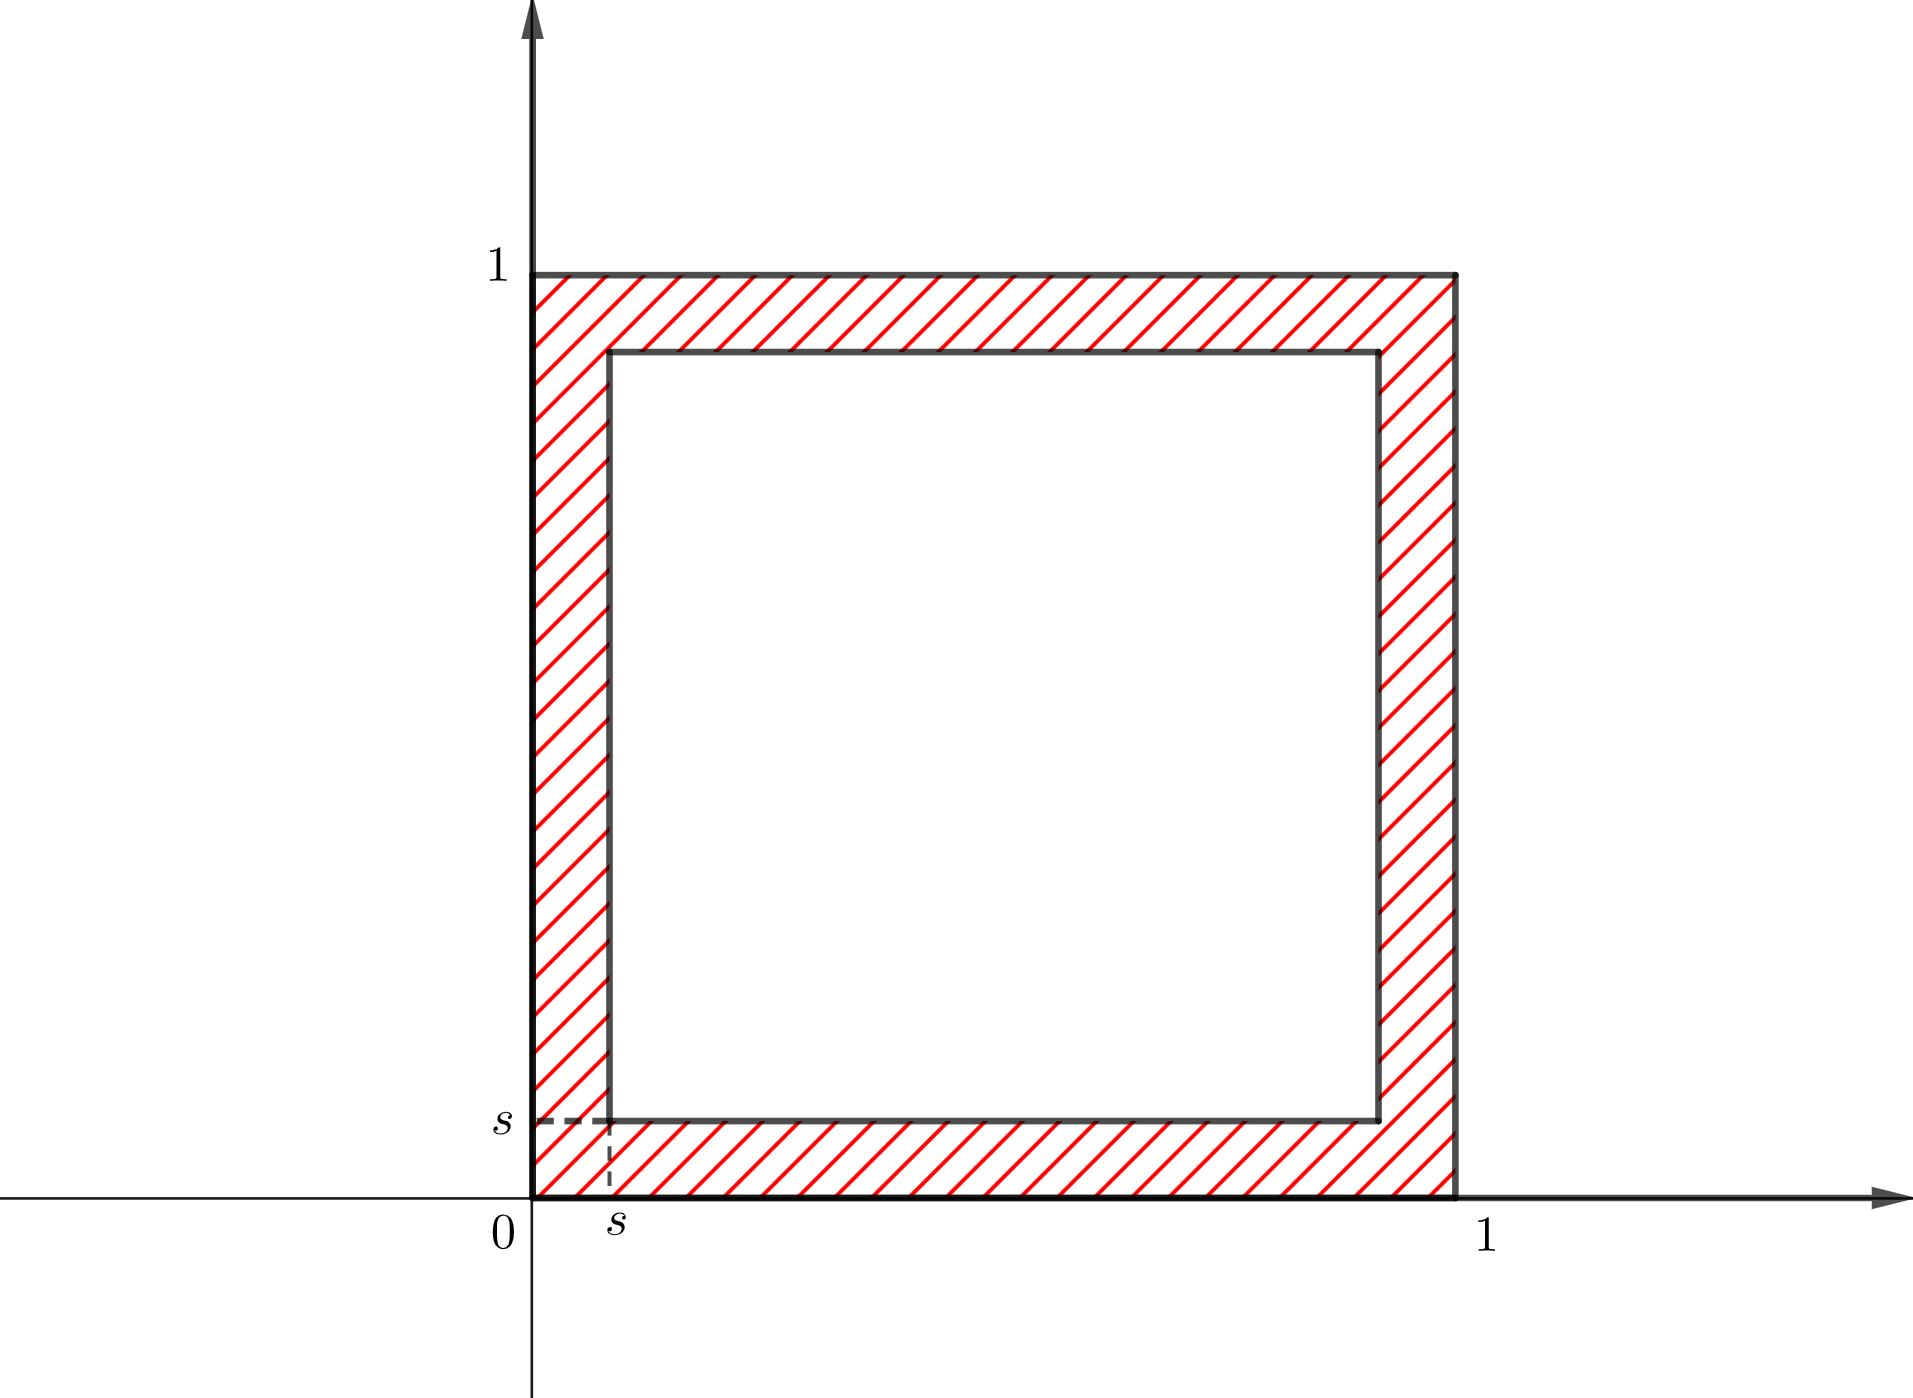
\includegraphics[scale=0.9]{tex/assets/prob-stat/software-engineering/SEM_kvadrat.png}
    \caption{Diagram for \textbf{Problem 1.1.}}
    \label{fig:enter-label}
\end{figure}

Thus $S$ is continuous with density $f(s)=4(1-2s)\one_{(0,1/2)}(s)$. If $F$ denotes the event of interest, $$\P(F)=\int_{-\infty}^{\infty}\underbrace{\P(F|S=s)}_{\pi s^2}f(s)\,ds=4\pi\int_0^{1/2}(s^2-2s^3)\,ds=\frac{\pi}{24}.$$

\begin{enumerate}[resume]
    \item (0.5 points) Let $X\sim\mbox{Unif}(0,1)$ and $Y:=X(1-X)$. Find $f_Y,F_Y,\mathbb E[Y],\mbox{Var}(Y)$.
\end{enumerate}
The function $g(x)=x(1-x)$ is not monotone, so the change-of-variables formula cannot be applied directly. It is monotone on $[0,1/2]$ and $[1/2,1]$. Apply the formula on each interval and add the resulting densities.

On $[0,1/2]$, the inverse is $h_1(y)=\frac12-\frac12\sqrt{1-4y}$ for $y\in[0,1/4]$; on $[1/2,1]$, it is $h_2(y)=\frac12+\frac12\sqrt{1-4y}$ on the same range (see below).

For $y\in[0,1/4]$, $$f_Y(y)=f_1(y)+f_2(y)=f_X(h_1(y))|h'_1(y)|+f_X(h_2(y))|h'_2(y)|.$$
$$= \one_{(0, 1)}(h_1(y)).\frac{1}{\sqrt{1-4y}}+\one_{(0, 1)}(h_2(y)).\frac{1}{\sqrt{1-4y}}.$$
It remains to determine where the indicators equal 1. The equation $\one_{(0,1)}(h_i(y))=1$, $i\in\{1,2\}$, is equivalent to $0<1+(-1)^i\sqrt{1-4y}<2$, which holds whenever $y\in(0,1/4)$. Hence $$f_Y(y)=\frac{2}{\sqrt{1-4y}}\one_{(0,1/4)}(y).$$

\vfill
\newpage

\begin{figure}[h]
    \centering
    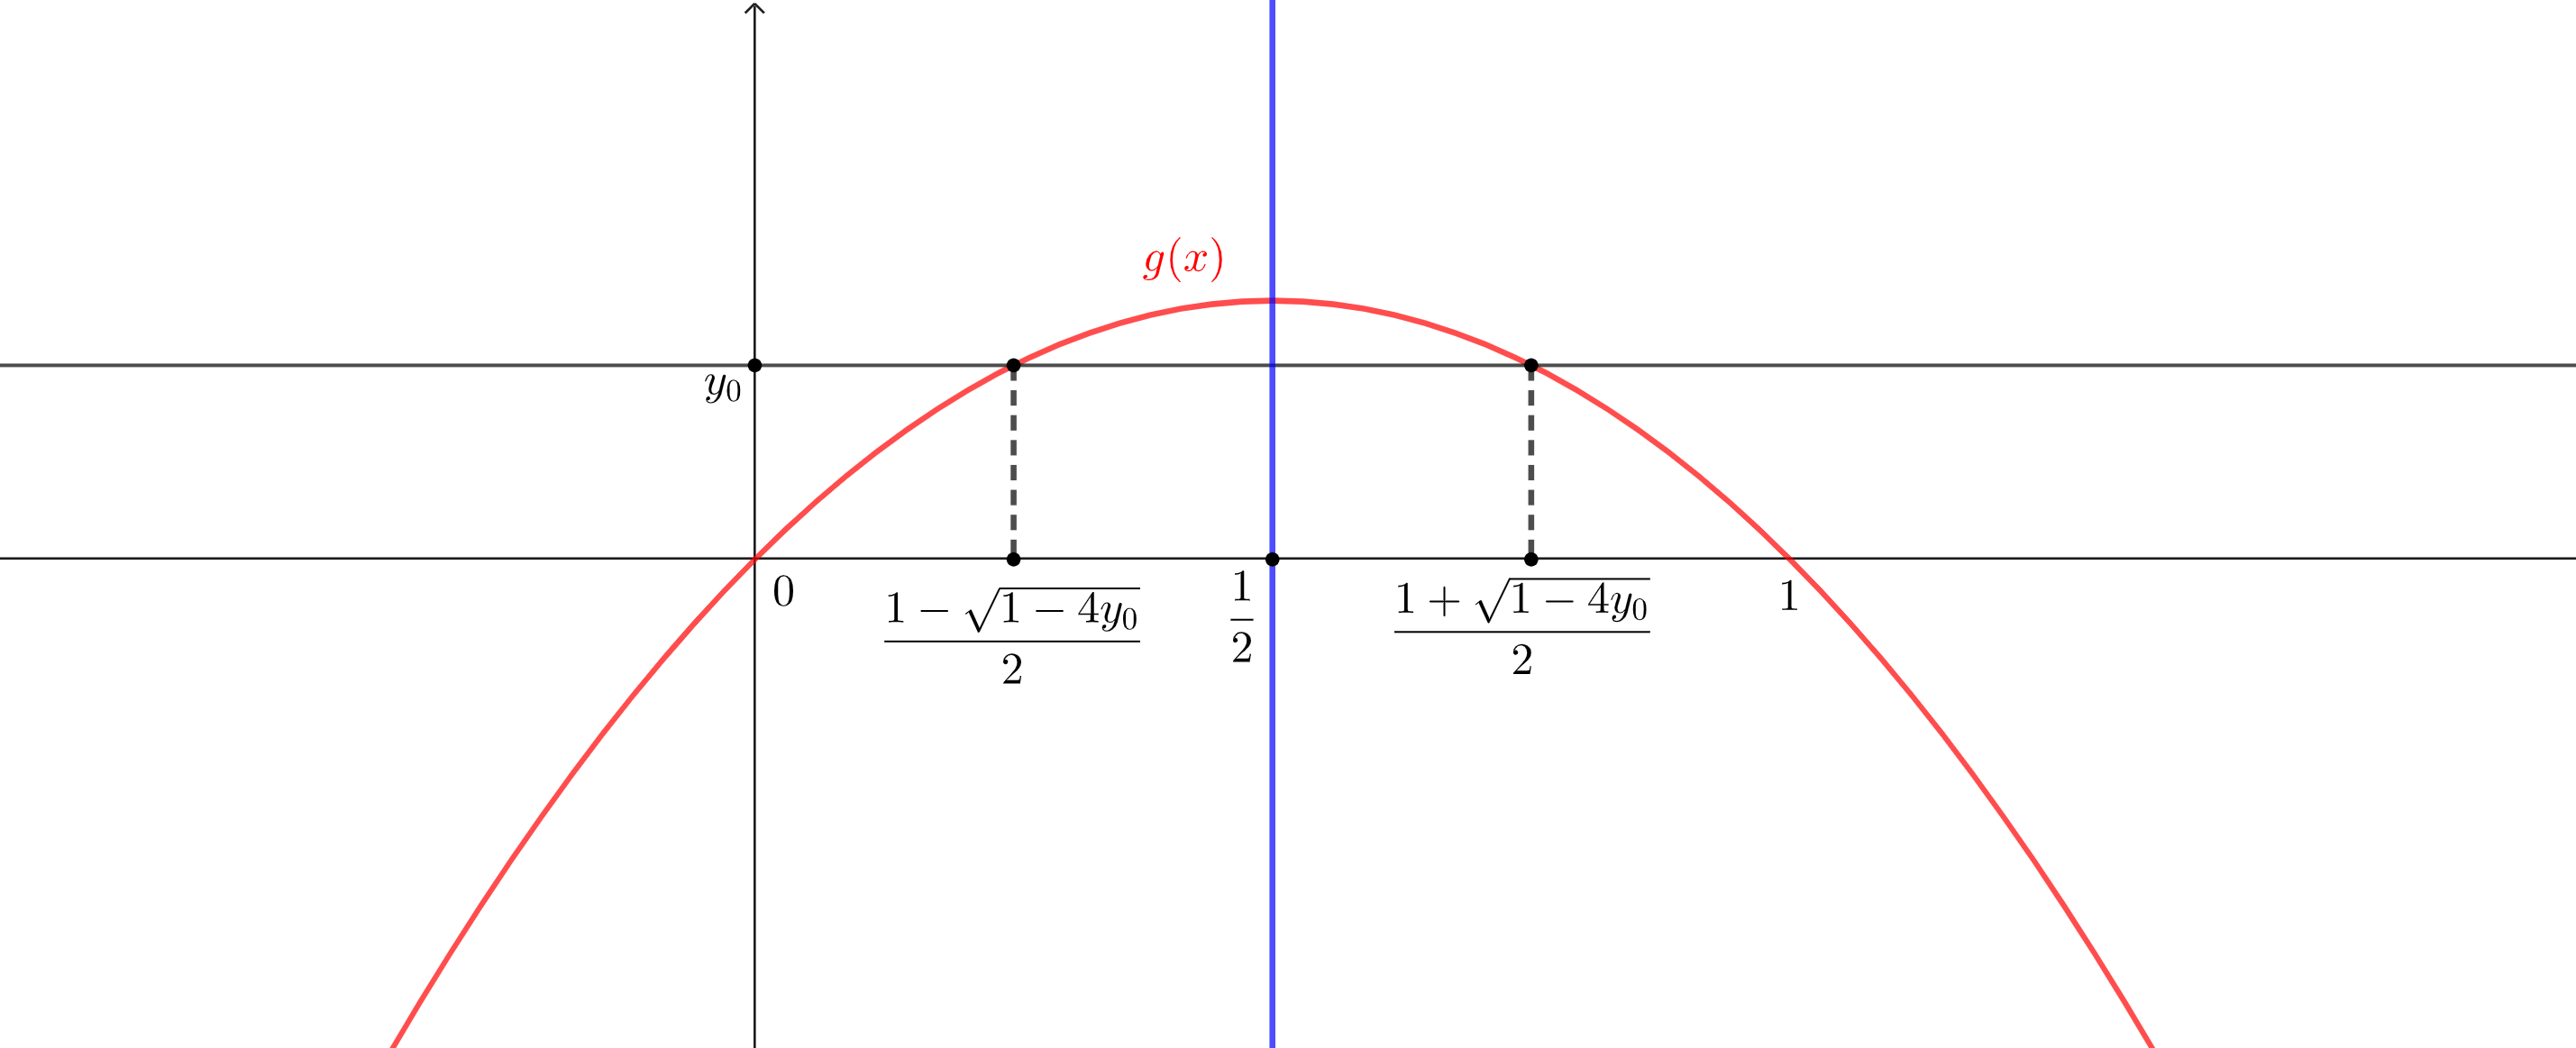
\includegraphics[scale=6]{tex/assets/prob-stat/software-engineering/sm_prom.png}
    \caption{Diagram for \textbf{Problem 1.2.}}
    \label{fig:enter-label}
\end{figure}

Alternatively, for $y\in[0,1/4]$,
$$F_Y(y)=\P(Y\leq y) = \P\left(X(1-X)\leq y, X\leq 1/2\right)+\P\left(X(1-X)\leq y, X> 1/2\right)$$
$$= \P\left(X\leq\frac{1-\sqrt{1-4y}}{2}\right)+\P\left(X>\frac{1+\sqrt{1-4y}}{2}\right) = \frac{1-\sqrt{1-4y}}{2}+1-\frac{1+\sqrt{1-4y}}{2}=1-\sqrt{1-4y}$$
For $y<0$, $F_Y(y)=0$, and for $y>1/4$, $F_Y(y)=1$. We can also obtain $f_Y=F_Y'$ almost everywhere this way. Furthermore, $\E Y=\E X-\E X^2=1/6$, $\E Y^2=\E[X^2(1-X)^2]=\E[X^2-2X^3+X^4]=1/30$, and $\mbox{Var}(Y)=1/180$.

\begin{enumerate}[resume]
    \item (0.5 points) Let $X,Y$ have joint density
\[f_{XY}(x,y):=\left\{\begin{array}{cc}
     c(x+y),  & x\geq0, y\geq0, x+y\leq 1 \\
     0, &\mbox{otherwise}.
\end{array}\right. \]
Define the random variables
\[U:=X+Y,\qquad V:=1-\frac{Y}{U}.\]
Find $f_{U,V}$, $\mbox{Cov}(U,V)$, $\mathbb E[X|U]$ and $\mathbb E[U|Y]$.
\end{enumerate}

For $c$, $$1=\iint f_{X,Y}(x,y)\,dx\,dy=\int_0^1\int_0^{1-x}c(x+y)\,dy\,dx=c\int_0^1\left(x-x^2+\frac{(1-x)^2}{2}\right)\,dx=\frac c3.$$ Thus $c=3$. Consider $(x,y)\mapsto(x+y,1-y/(x+y))=(x+y,x/(x+y))$, whose inverse is $(u,v)\mapsto(uv,u-uv)$. Its Jacobian is $$J=\begin{vmatrix}
v & u \\
1-v & -u
\end{vmatrix}=-u\neq0\quad\textrm{for }x,y\in D_{X,Y}\setminus\{(0,0)\}.$$ The transformation formula gives
$$f_{U, V}(u, v) = f_{X, Y}(uv, u-uv).|J| = 3(uv+u-uv).|u|.\one_{\{0\leq uv\leq 1, ~0\leq u-uv\leq 1-uv\}}.$$

The support requires $0\leq uv\leq1$ and $uv\leq u\leq1$, i.e. $0\leq uv\leq u\leq1$. Thus $0\leq u,v\leq1$ (which automatically implies $uv\leq u$). Hence $f_{U,V}(u,v)=3u^2\one_{(0,1)^2}(u,v)$. The density does not depend on $v$ except through its support. Its marginal densities are $f_V(v)=\one_{(0,1)}(v)$, so $V\sim\mbox{Unif}(0,1)$, and $f_U(u)=3u^2\one_{(0,1)}(u)$. Hence $U\indep V$ because $f_{U,V}=f_Uf_V$, and $\mbox{Cov}(U,V)=0$.

For the conditional expectations, use conditional densities. The transformation $(x,y)\mapsto(x,x+y)$ gives $$f_{X,U}(x,u)=f_{X,Y}(x,u-x)\begin{vmatrix}
1 & 0 \\
-1 & 1
\end{vmatrix}=3(x+u-x)\one_{(0,1)}(u-x)\one_{(0,1-(u-x))}(x)=3u\one_{(0,1)}(u)\one_{(0,u)}(x).$$ Since $f_U(u)=3u^2\one_{(0,1)}(u)$, for $u\in(0,1)$, $$f_{X|U}(x|u)=\frac{3u\one_{(0,u)}(x)}{3u^2}=u^{-1}\one_{(0,u)}(x).$$
Now $$\E[X|U=u]=\int_{-\infty}^{\infty}xf_{X|U}(x|u)\,dx=\int_0^u\frac{x}{u}\,dx=\frac u2$$ for $u\in(0,1)$. Thus $\E[X|U]=U/2$ (see below). Alternatively, $\Ebb{X|U}=\Ebb{UV|U}=U\Ebb V=U/2$.
For the second expectation, $\E[X+Y|Y]=\E[X|Y]+\E[Y|Y]=\E[X|Y]+Y$, so it suffices to calculate $\E[X|Y]$.
$$f_Y(y) = \int\limits_{0}^{1-y}3(x+y)dx~.\one_{(0, 1)}(y) = \frac{3}{2}\left(1-y^2\right).\one_{(0, 1)}(y),$$
$$\Rightarrow f_{X|Y}(x|y) = \left\{\begin{array}{cc}
     \frac{3(x+y)}{3/2(1-y^2)}\cdot\one_{(0, 1-y)}(x),  & y\in(0, 1) \\
     0, &\mbox{otherwise}.
\end{array}\right.$$
Therefore $$\E[X|Y=y]=\int_0^{1-y}x\frac{2x+2y}{1-y^2}\,dx=\frac{2}{3(1-y^2)}x^3\bigg|_0^{1-y}+\frac{y}{1-y^2}x^2\bigg|_0^{1-y}=\frac{2-y-y^2}{3+3y},$$
so $$E[U|Y]=\frac{2-Y-Y^2}{3+3Y}+Y=\frac23\frac{1+Y+Y^2}{1+Y}.$$

\begin{figure}[h]
    \centering
    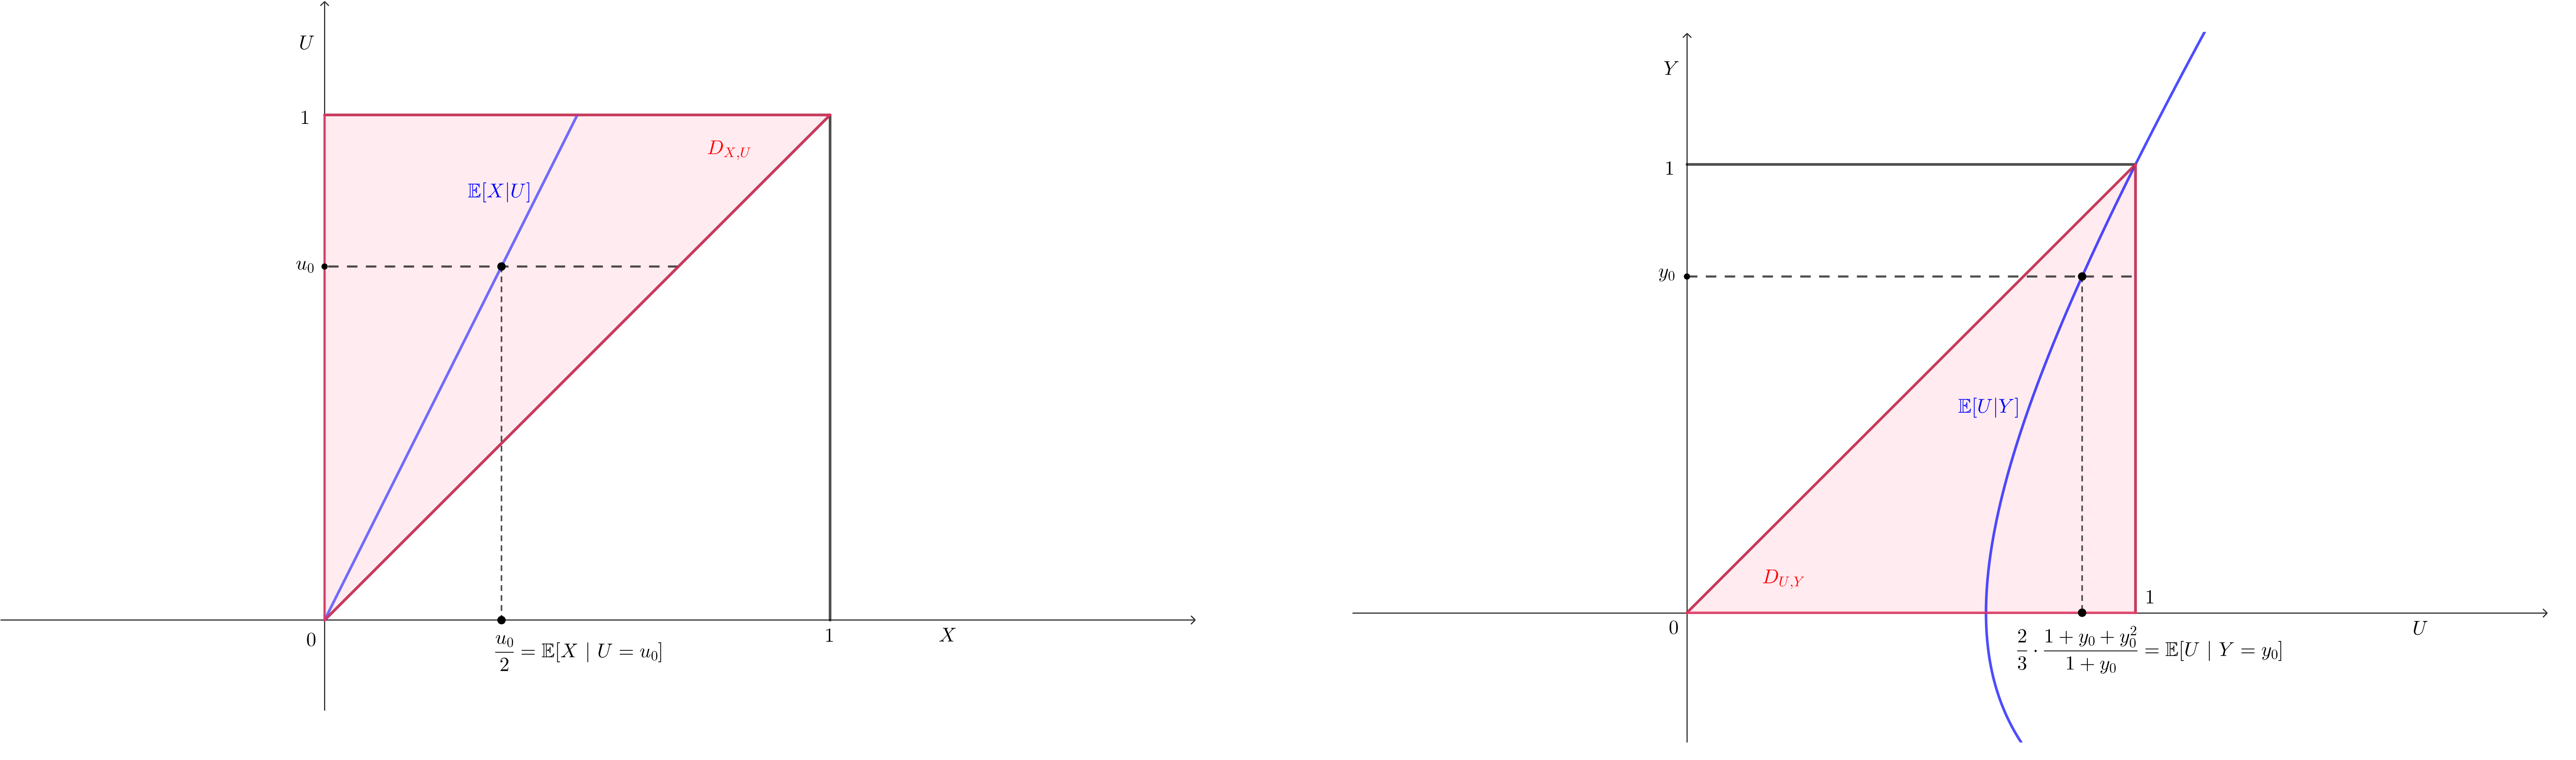
\includegraphics[scale=3.25]{tex/assets/prob-stat/software-engineering/SEM_cond_exp_1.png}
    \caption{The conditional expectations $\E[X|U]$ and $\E[U|Y]$ are shown in \textcolor{blue}{blue}.}
    \label{fig:enter-label}
\end{figure}

\end{problem}

\begin{problem}
A metro station has an electronic timetable display with $48\times40$ LEDs. Their lifetimes are independent exponential variables with mean 40,000 operating hours. The display operates 18 hours daily. If fewer than $85\%$ of the LEDs work, the text becomes hard to read and the display must be replaced.
\begin{enumerate}
    \item (0.25 points) Approximate the probability that the display needs replacement after 365 days.
\end{enumerate}
Let $X_i$ be the lifetime in hours of LED $i$, $1\leq i\leq48\times40$. The $X_i$ are iid $\mbox{Exp}(1/40\,000)$. The number working at time $t$ is $$T_t=\sum_{i=1}^{48\times40}\one_{\{X_i\geq t\}}\sim\mbox{Bin}(48\times40,\P(X_i\geq t)).$$
Replacement after 365 days at 18 hours daily means $T_{365\times18}<85\%\times48\times40=1632$. Here $p=\Pbb{X_i\geq365\times18}=\exp(-365\times18/40\,000)$. Thus $\mu=\Ebb{T_{365\times18}}=48\times40\exp(-365\times18/40\,000)\approx1629.18$ and $\sigma=\sqrt{\mbox{Var}(T_{365\times18})}=\sqrt{\mu(1-p)}\approx15.71$. The CLT gives the approximation
$$\Pbb{T_{365\times18}<85\%\times48\times40} \approx \Pbb{\frac{T_{365\times18}-\mu}{\sigma}<\frac{1632-1629.18}{15.71}}\approx \Phi(0.1795)\approx 57.142\%.$$

\begin{enumerate}[resume]
    \item (0.5 points) Let $T_{min}$ be the time in operating hours to the first LED failure. Find its distribution and $\mathbb E[T_{min}]$, the probability of the first failure within $k$ calendar days, and its median.
\end{enumerate}
We have $T_{min}=\min\{X_i:1\leq i\leq48\times40\}$. For independent $X\sim\mbox{Exp}(\alpha)$ and $Y\sim\mbox{Exp}(\beta)$, $\min\{X,Y\}\sim\mbox{Exp}(\alpha+\beta)$, since $\Pbb{\min\{X,Y\}>t}=\Pbb{X>t}\Pbb{Y>t}=e^{-\alpha t}e^{-\beta t}=e^{-(\alpha+\beta)t}$. Together with $\min\{X_i:1\leq i\leq n\}=\min\{X_n,\min\{X_i:1\leq i\leq n-1\}\}$, this yields $T_{min}\sim\mbox{Exp}(48\times40/40\,000)$ and $\Ebb{T_{min}}=40\,000/(48\times40)\approx20.83$.
$$\Pbb{T_{min} \leq 18k} = 1-e^{-48\times40\times18k/40~000}.$$

For an exponential variable of rate $\lambda>0$, the median $m$ satisfies
$$\frac{1}{2} = \Pbb{X\leq m} = 1-e^{-\lambda m}~~\Rightarrow~~-\lambda m = -\ln2~~\Rightarrow~~ m=\frac{\ln2}{\lambda}\cdot$$
In particular, the median of $T_{min}$ is $(40\,000\ln2)/(48\times40)\approx14.44$.
\begin{enumerate}[resume]
    \item (0.5 points) After 12 months, exactly 1700 LEDs are found working. What is the distribution of the remaining lifetime of an individual LED at this time? Find the probability that the display becomes unreadable within the next three months.
\end{enumerate}
It is natural to ask about the lifetime of LED $i$ if it \emph{has not failed} at time $t$ (here $t=365\times18$). For $s>0$, $$\Pbb{X_i>t+s|T_t=1700}=\frac{\Pbb{X_i>t+s,T_t=1700}}{\Pbb{T_t=1700}}=\frac{\Pbb{X_i>t+s,\sum_{j\neq i}\one_{\{X_j\geq t\}}=1699}}{\Pbb{T_t=1700}},$$ because $X_i>t+s$ implies $\one_{\{X_i\geq t\}}=1$. Mutual independence allows the numerator to factor: $$\Pbb{X_i>t+s|T_t=1700}=\frac{\Pbb{X_i>t+s}\Pbb{T_t^{(i)}=1699}}{\Pbb{T_t=1700}},$$ where $T_t^{(i)}=T_t-\one_{\{X_i\geq t\}}$, so $T_t^{(i)}\sim\mbox{Bin}(n-1,p)$\footnote{Here $p=\Pbb{X_1\geq t}=e^{-t/40\,000}$ and $n=48\times40$.}. Calculate:
$$\Pbb{X_i>t+s~|~T_t=1700} = \frac{e^{-(t+s)/40~000}\binom{n}{1699}p^{1699}(1-p)^{n-1699}}{\binom{n}{1700}p^{1700}(1-p)^{n-1700}}$$
$$= \frac{1700}{n-1699}\cdot\frac{1-p}{p}\cdot e^{-(t+s)/40~000} = \frac{1700}{221}\left(e^{-s/40~000}-e^{-(t+s)/40~000}\right),$$
The density conditional on $\{T_t=1700\}$ can also be obtained from this.

One could also ask about the conditional distribution of the time $\widetilde X_i$ to failure for an LED that \emph{has already failed} at $t$. For $0<s<t$, $$\Pbb{\widetilde X_i<-s|T_t=1700}=\Pbb{X_i<t-s|T_t=1700}=\frac{\Pbb{X_i<t-s}\Pbb{T_t^{(i)}=1700}}{\Pbb{T_t=1700}},$$ again using independence and the fact that $X_i<t-s$ implies $\one_{\{X_i\geq t\}}=0$. This can be calculated similarly.

For the final question, calculate $\Pbb{T_{t+90\times18}<1632|T_t=1700}$, where $t=365\times18$. More than 68 LEDs must fail in those three months (so $t\leq X_i<t+90\times18$ for them). Writing $F(t)=\Pbb{X_1>t|T_t=1700}$ as calculated above, the required probability is
$$\sum_{k=69}^{1700}{\binom{1700}{k}\left(1-F(t+90\times18)\right)^k\left(F(t+90\times18)\right)^{1700-k}}.$$
\end{problem}
\vfill
\newpage
\begin{problem}
At a juice-bottling plant, the volume $X$ in one bottle (millilitres) is normally distributed with variance $\sigma^2=12^2$.
\begin{enumerate}
    \item (0.25 points) If $20\%$ of bottles contain less than 485 ml, find $\mu$. Find the percentage containing more than 525 ml.
\end{enumerate}
$$0.2 = \Pbb{X<485} = \Phi\left(\frac{485-\mu}{12}\right)~\Rightarrow~\frac{485-\mu}{12}\approx-0.84~\Rightarrow~\mu\approx495.08.$$
$$\Pbb{X>525} = 1-\Pbb{X\leq525} = 1-\Phi\left(\frac{525-495.08}{12}\right)\approx1-\Phi\left(2.493\right)=\Phi(-2.493)\approx 0.64\%.$$
\begin{enumerate}[resume]
    \item (0.25 points) After a production change, assume $X\sim\mbox N(505,\sigma^2)$. Find $\sigma$ if $95\%$ of bottles contain between 490 and 520 ml.
\end{enumerate}
$$0.95=\Pbb{490<X<520} = \Pbb{-\frac{15}{\sigma}<\frac{X-505}{\sigma}<\frac{15}{\sigma}} = \Phi\left(\frac{15}{\sigma}\right)-\Phi\left(-\frac{15}{\sigma}\right) = 1-2\Phi\left(-\frac{15}{\sigma}\right),$$
$$\Rightarrow \Phi\left(-\frac{15}{\sigma}\right)=0.025~\Rightarrow~-\frac{15}{\sigma}\approx-1.96~\Rightarrow~\sigma\approx 7.65.$$
\begin{enumerate}[resume]
    \item (0.5 points) After the change, with $\sigma$ from the preceding part, use two-stage quality control. First, randomly choose $n=30$ bottles from a batch and measure their volumes. Reject the batch if at least three contain under 490 ml. Otherwise, draw another $m=20$ bottles and calculate the mean volume of all $m+n=50$. Reject if this mean is below 503 ml, and accept otherwise. Find the rejection probability.
\end{enumerate}
Let $X_i$, $1\leq i\leq50$, be the volume in bottle $i$. As in Problem 2, put $$T=\sum_{i=1}^{30}\one_{\{X_i<490\}}\sim\mbox{Bin}(30,p),$$ where $p=\Pbb{X<490}=\Phi(-15/\sigma)=0.025$. Let $A$ be the event of rejecting the batch. Then $$\Pbb A=\Pbb{T\geq3}+\Pbb{T<3,\overline X_{50}<503}=1-\Pbb{T<3,\overline X_{50}\geq503}.$$
\end{problem}

\begin{problem} (0.75 points)
A server's load $Y$ is exponentially distributed with rate $\lambda>0$. Given $Y=y$, a task's processing time $X$ (seconds) is exponential with rate $y$. Find $f_X$, $\mathbb P(X>x)$, $\mathbb E[X]$ and the distribution of $X+Y$. Is $X+Y$ a continuous random variable?
\end{problem}
By assumption, $X|Y=y\sim\mbox{Exp}(y)$, so $f_{X|Y}(x|y)=ye^{-yx}\one_{(0,\infty)}(x)$. Hence $$f_{X,Y}(x,y)=f_Y(y)f_{X|Y}(x|y)=\lambda e^{-\lambda y}ye^{-yx}\one_{(0,\infty)}(x)\one_{(0,\infty)}(y)=\lambda ye^{-(\lambda+x)y}\one_{(0,\infty)^2}(x,y),$$ and the marginal density of $X$ for $x>0$ is
$$f_X(x)=\int_{-\infty}^{\infty}f_{X,Y}(x,y)\,dy=\int_0^\infty\lambda ye^{-(\lambda+x)y}\,dy=\color{red}\underbrace{\int_0^\infty y(\lambda+x)e^{-(\lambda+x)y}\,dy}_{(\lambda+x)^{-1}}\color{black}-x\int_0^\infty ye^{-(\lambda+x)y}\,dy=$$\footnote{The first integral is the expectation of an exponential random variable with rate $\lambda+x$.}
$$= \frac{1}{\lambda+x}+\underbrace{\frac{x}{\lambda+x}ye^{-(\lambda + x)y}\bigg\rvert_{y=0}^{\infty}}_{0}-\frac{x}{\lambda+x}\int\limits_{0}^{\infty}e^{-(\lambda + x)y}dy =\frac{1}{\lambda+x}+\frac{x}{(\lambda+x)^2}e^{-(\lambda + x)y}\bigg\rvert_{y=0}^{\infty} = \frac{\lambda}{(\lambda+x)^2}\cdot$$
Thus, for $x>0$, $$\P(X>x)=\int_x^\infty\frac{\lambda}{(\lambda+t)^2}\,dt=\frac{\lambda}{\lambda+t}\bigg|_\infty^x=\frac{\lambda}{\lambda+x},\qquad \E X=\int_0^\infty\frac{\lambda x}{(\lambda+x)^2}\,dx=+\infty,$$
because the last integral diverges. For the distribution of $X+Y$, when $s>0$,
\begin{align*}
\P(X+Y\leq s)
&=\int_{-\infty}^\infty\P(X+Y\leq s|Y=y)f_Y(y)\,dy\\
&=\int_0^\infty\P(X+y\leq s|Y=y)\lambda e^{-\lambda y}\,dy\\
&=\int_0^s(1-e^{-y(s-y)})\lambda e^{-\lambda y}\,dy.
\end{align*} The last equality uses $\P(X+y\leq s|Y=y)=0$ when $y>s$, and the exponential conditional law, giving $\P(X\leq s-y|Y=y)=1-e^{-y(s-y)}$. The CDF is differentiable for $s>0$, zero for $s\leq0$, and continuous at 0, hence absolutely continuous. Thus $X+Y$ is continuous with density $$f_{X+Y}(s)=\frac{d}{ds}F_{X+Y}(s)=\frac{d}{ds}\left(\int_0^s(1-e^{-y(s-y)})\lambda e^{-\lambda y}\,dy\right)\one_{(0,\infty)}(s)=$$
$$\left(\left(1-e^{-y(s-y)}\right)\lambda e^{-\lambda y}\bigg\rvert_{y=s}+\int\limits_{0}^{s}\frac{\partial}{\partial s}\left(1-e^{-y(s-y)}\right)\lambda e^{-\lambda y}dy\right)~\one_{(0, \infty)}(s) = \int\limits_{0}^{s}ye^{-y(s-y)}\lambda e^{-\lambda y}dy.~\one_{(0, \infty)}(s).$$

\end{document}
